\KOMAoptions{paper=A3}
\recalctypearea
\subsection{Thue-Morse Sequence}{\label{pp:thuemorsesequence}}
Thue-Morse Sequence aka Fair Share Sequence is an infinite binary sequence obtained by starting with 0 and successively appending the Boolean complement of the sequence obtained thus far (called prefixes of the sequence).\\
For example, starting with the sequence \textbf{0},
\begin{itemize}
	\item Append complement of \textbf{0}, we get 0\textbf{1}
	\item Append complement of \textbf{01}, we get 01\textbf{10}
	\item Append complement of \textbf{0110}, we get 0110\textbf{1001} and so on.
\end{itemize}
Also, by using Thue-Morse sequence elements in the turtle simulator, we get a mysterious curve\footnote{called Koch curve, it is a fractal curve that has infinite length but contained in a finite area. Can you see why?} by following the below rule.
\begin{itemize}
	\item If an element is 0, then the turtle rotates \verb!right! by 180\textdegree.
	\item If an element is 1, then the turtle moves \verb!forward! by one unit and then rotates \verb!right! by 60\textdegree.
\end{itemize}
Can you figure out the pattern of this curve?

\textbf{Problem Statement:}\\
Generate the first $n$ elements of the Thue-Morse sequence and draw the corresponding curve using \verb!turtleSim!.\\
Scale the curve in such a way that it roughly takes same width and height for all $n$.
% \begin{testcasesMore}
% 	{$t$ \hfill(number of test cases, an integer)\\
% 	$n_1\ n_2\ \ldots n_t$ \hfill($t$ space seperated integers for each testcase)}
% 	{First $n_i$ elements of the Thue-Morse sequence and the curve.\hfill(each testcase on a newline)}
% 	{$1 \leq n_i \leq 100000$ ($n_i$ need not be a power of 2)}
% 	{4\\2 32 111 128}
% 	{01\\01101001100101101001011001101001\\011010011001011010010110011010011001011001101001011010011001011010010110011010010110100110010110011010011001011\\01101001100101101001011001101001100101100110100101101001100101101001011001101001011010011001011001101001100101101001011001101001}
% 	{https://github.com/paramrathour/CS-101/tree/main/Test Cases/Thue-Morse Sequence/Input.txt}
% 	{https://github.com/paramrathour/CS-101/tree/main/Test Cases/Thue-Morse Sequence/Output.txt}
% 	{https://github.com/paramrathour/CS-101/tree/main/Starter Codes/Thue-Morse Sequence.cpp}
% \end{testcasesMore}
\begin{testcasesMore}
	{$n$ \hfill(a single integer)}
	{First $n$ elements of the Thue-Morse sequence and the curve.}
	{$1 \leq n \leq 100000$ ($n$ need not be a power of 2)}
	{111}
	{011010011001011010010110011010011001011001101001011010011001011010010110011010010110100110010110011010011001011}
	{https://github.com/paramrathour/CS-101/tree/main/Test Cases/Thue-Morse Sequence/Input.txt}
	{https://github.com/paramrathour/CS-101/tree/main/Test Cases/Thue-Morse Sequence/Output.txt}
	{https://github.com/paramrathour/CS-101/tree/main/Starter Codes/Thue-Morse Sequence.cpp}
\end{testcasesMore}
\textbf{The output Koch Curve convergents}
\begin{figure}[H]
	\centering
	\begin{subfigure}{0.3\linewidth}
		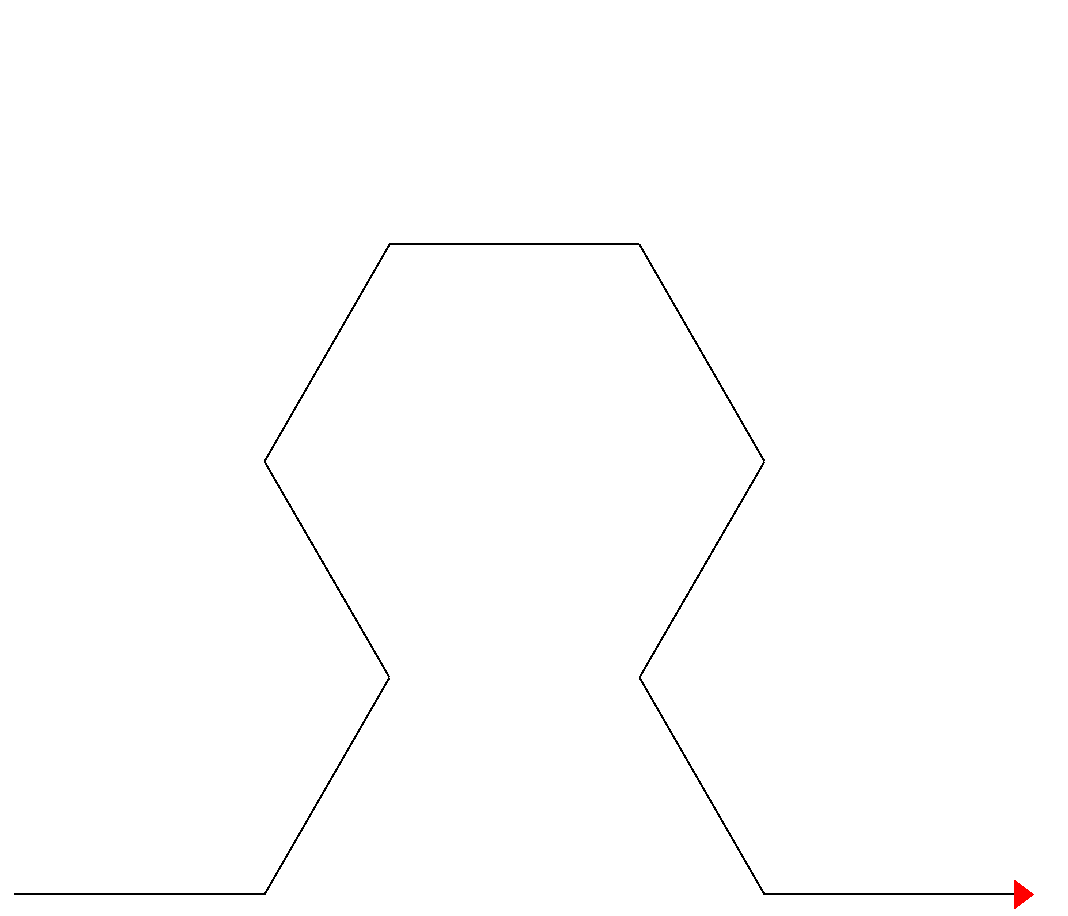
\includegraphics[width = \linewidth]{Thue-Morse Sequence/2.png}
		\caption{Iteration 0, $n=2$}
	\end{subfigure}
	\begin{subfigure}{0.3\linewidth}
		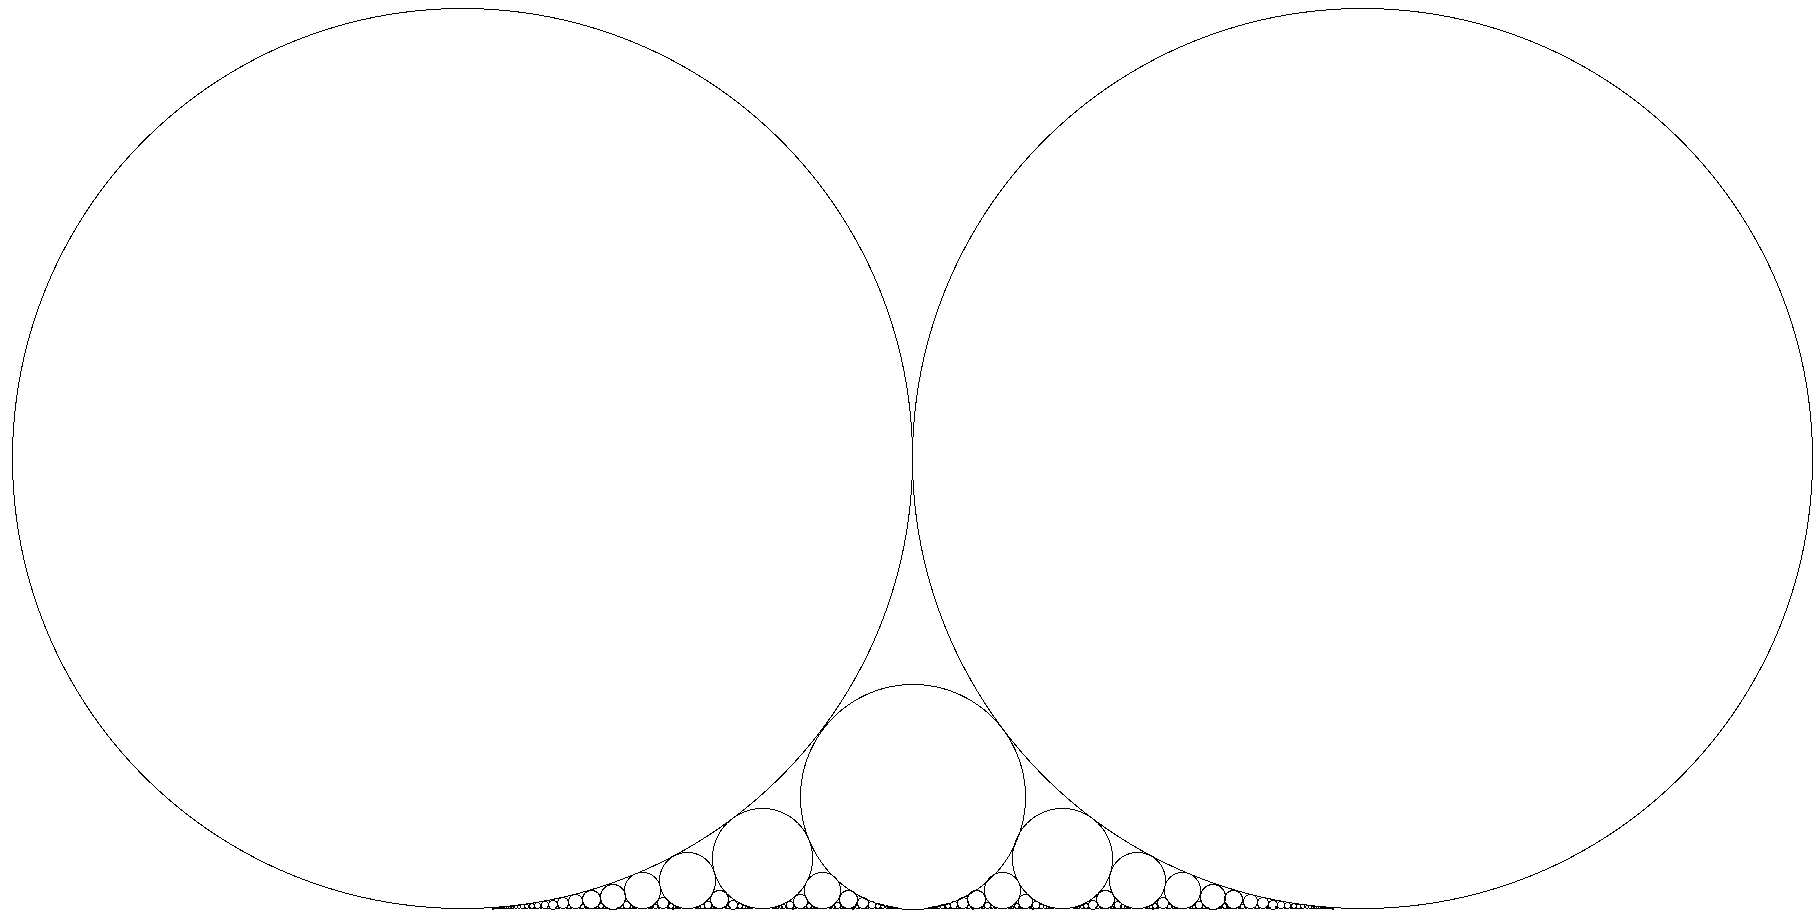
\includegraphics[width = \linewidth]{Thue-Morse Sequence/8.png}
		\caption{Iteration 1, $n=8$}
	\end{subfigure}
	\begin{subfigure}{0.3\linewidth}
		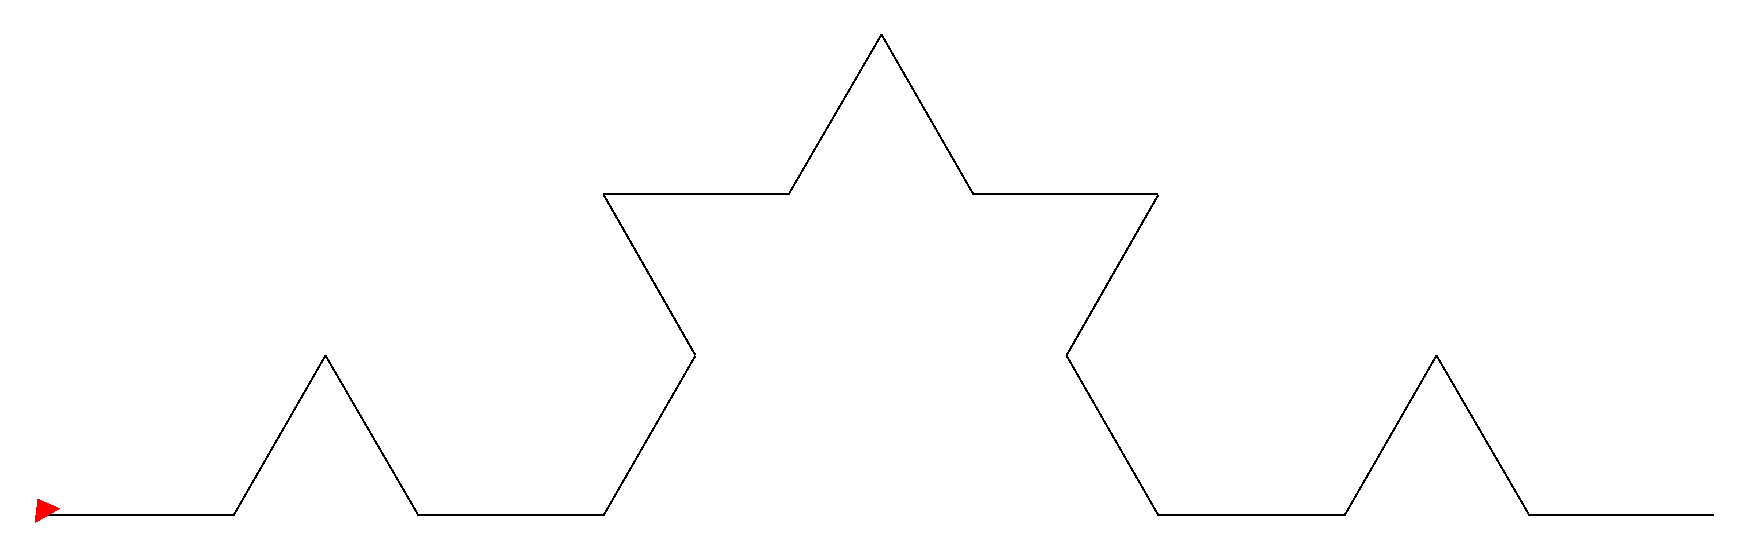
\includegraphics[width = \linewidth]{Thue-Morse Sequence/32.png}
		\caption{Iteration 2, $n=32$}
	\end{subfigure}
	\begin{subfigure}{0.3\linewidth}
		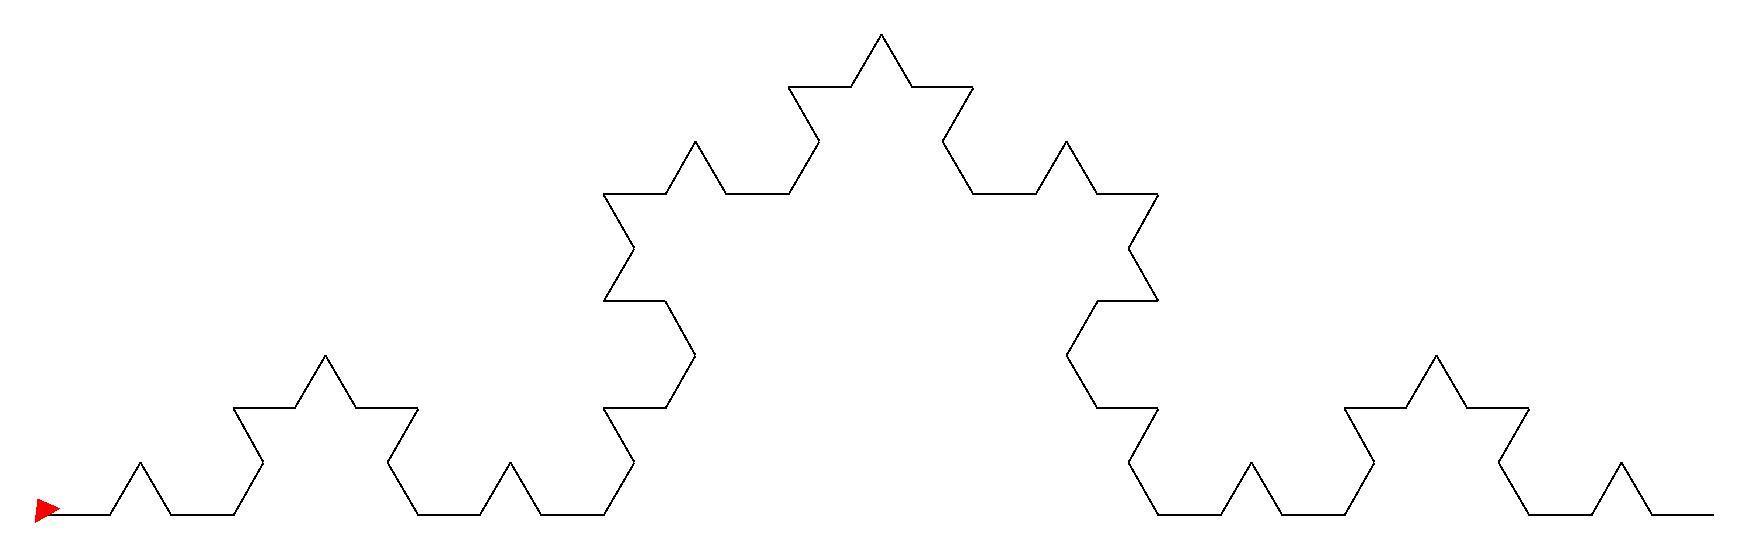
\includegraphics[width = \linewidth]{Thue-Morse Sequence/128.png}
		\caption{Iteration 3, $n=128$}
	\end{subfigure}
	\begin{subfigure}{0.3\linewidth}
		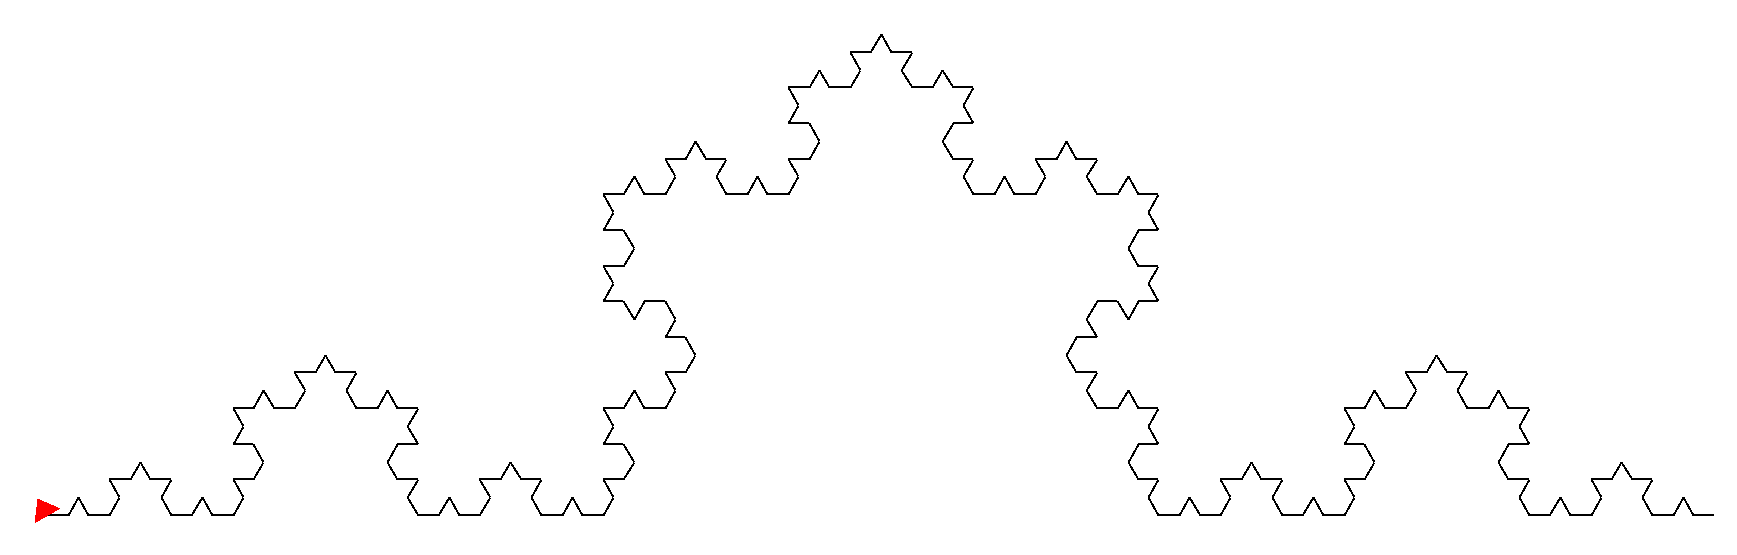
\includegraphics[width = \linewidth]{Thue-Morse Sequence/512.png}
		\caption{Iteration 4, $n=512$}
	\end{subfigure}
	\begin{subfigure}{0.3\linewidth}
		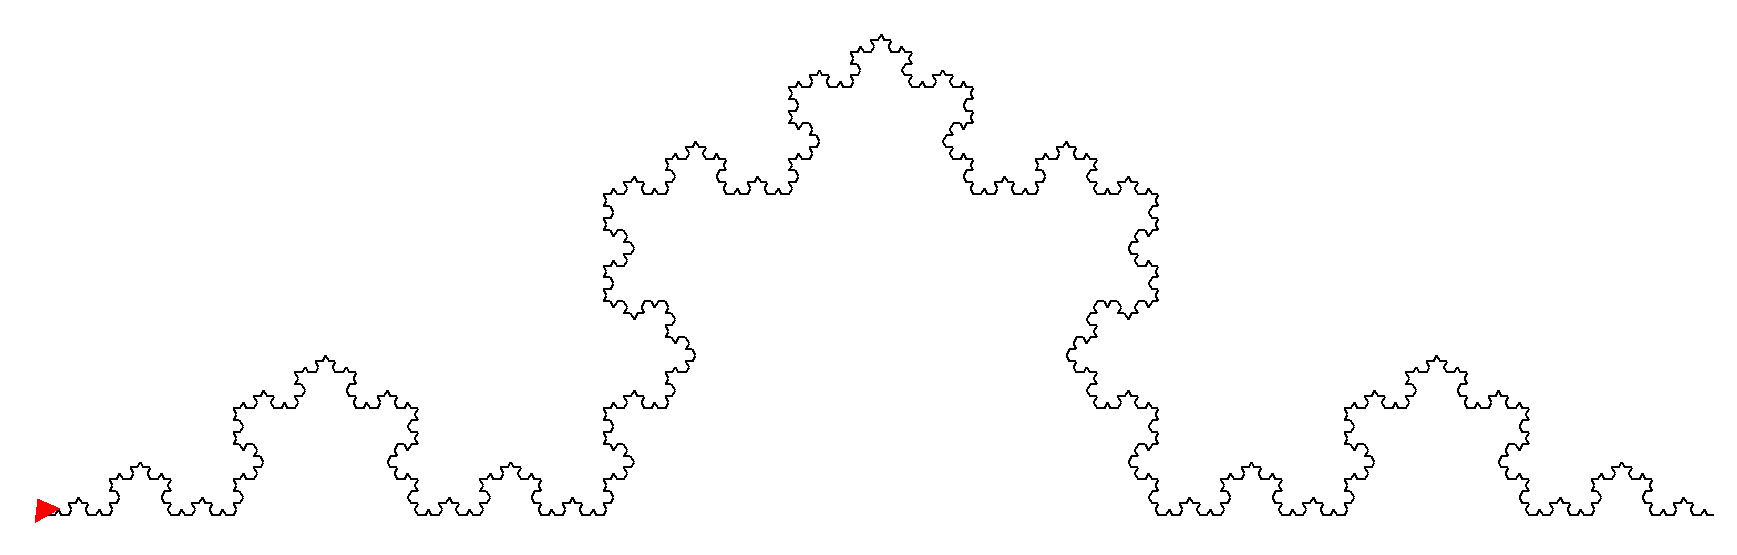
\includegraphics[width = \linewidth]{Thue-Morse Sequence/2048.png}
		\caption{Iteration 5, $n=2048$}
	\end{subfigure}
	\begin{subfigure}{0.3\linewidth}
		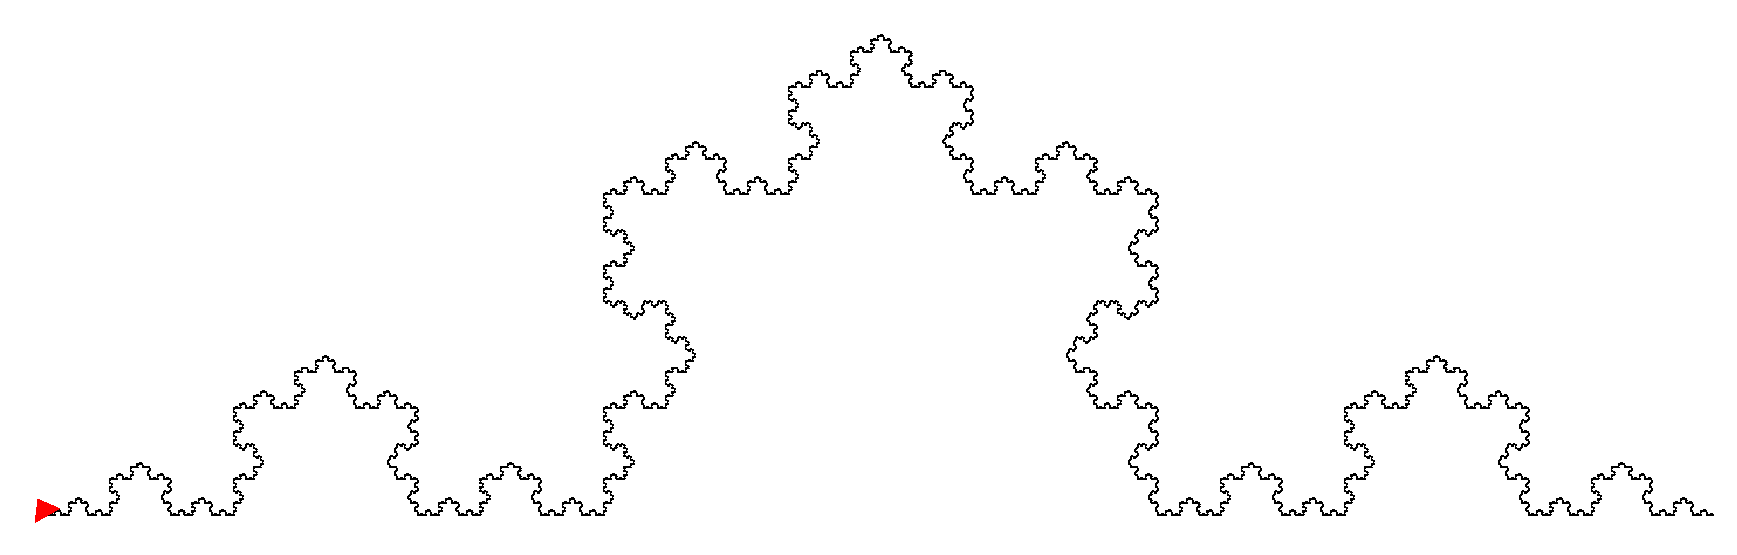
\includegraphics[width = \linewidth]{Thue-Morse Sequence/8192.png}
		\caption{Iteration 6, $n=8192$}
	\end{subfigure}
	\caption{Koch Curve Iterations and the outputs for odd powers of 2}
\end{figure}
\begin{figure}[H]
	\centering
	\begin{subfigure}{0.3\linewidth}
		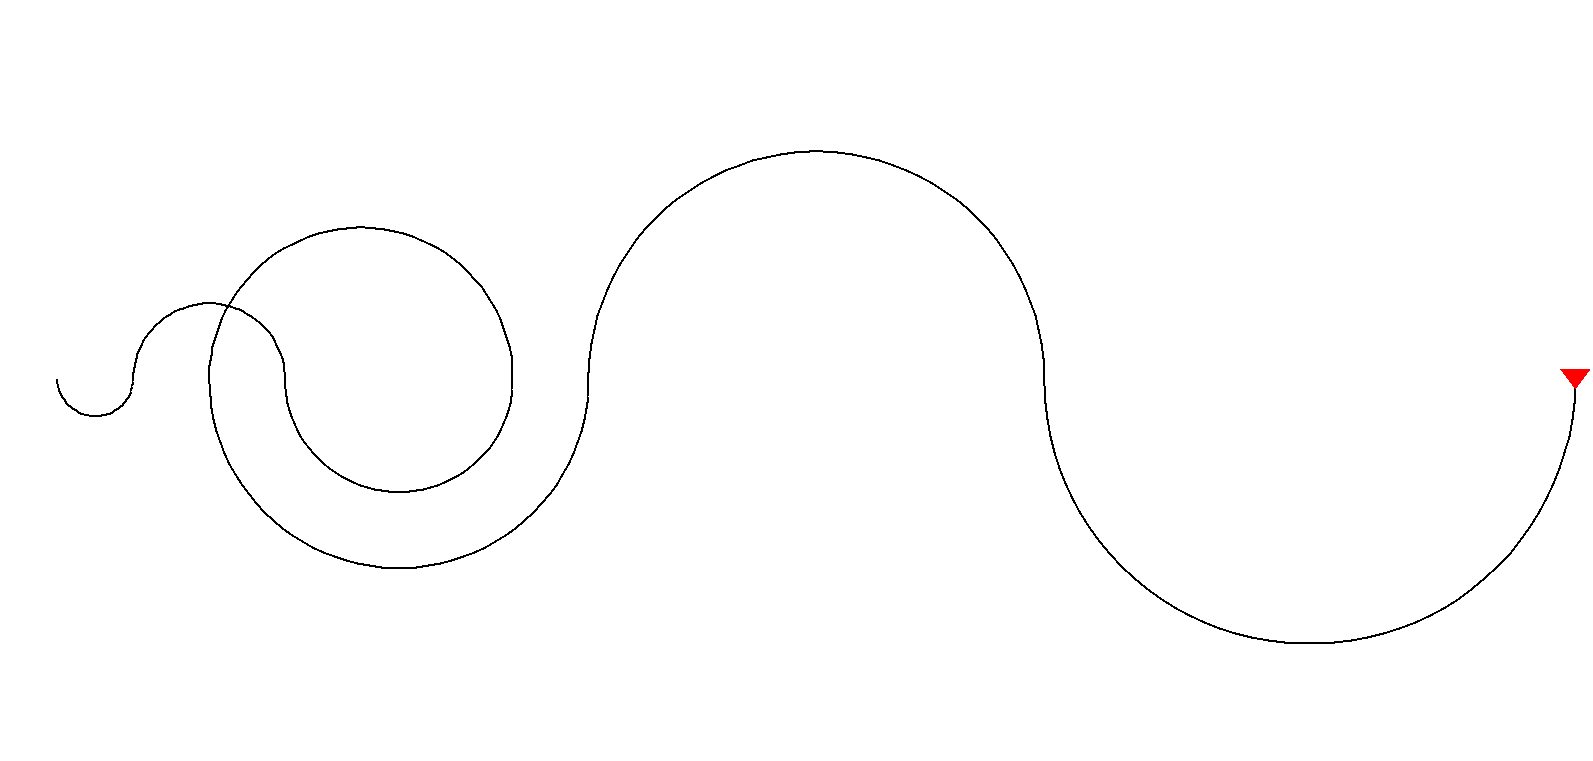
\includegraphics[width = \linewidth]{Thue-Morse Sequence/4.png}
		\caption{$n=4$}
	\end{subfigure}
	\begin{subfigure}{0.3\linewidth}
		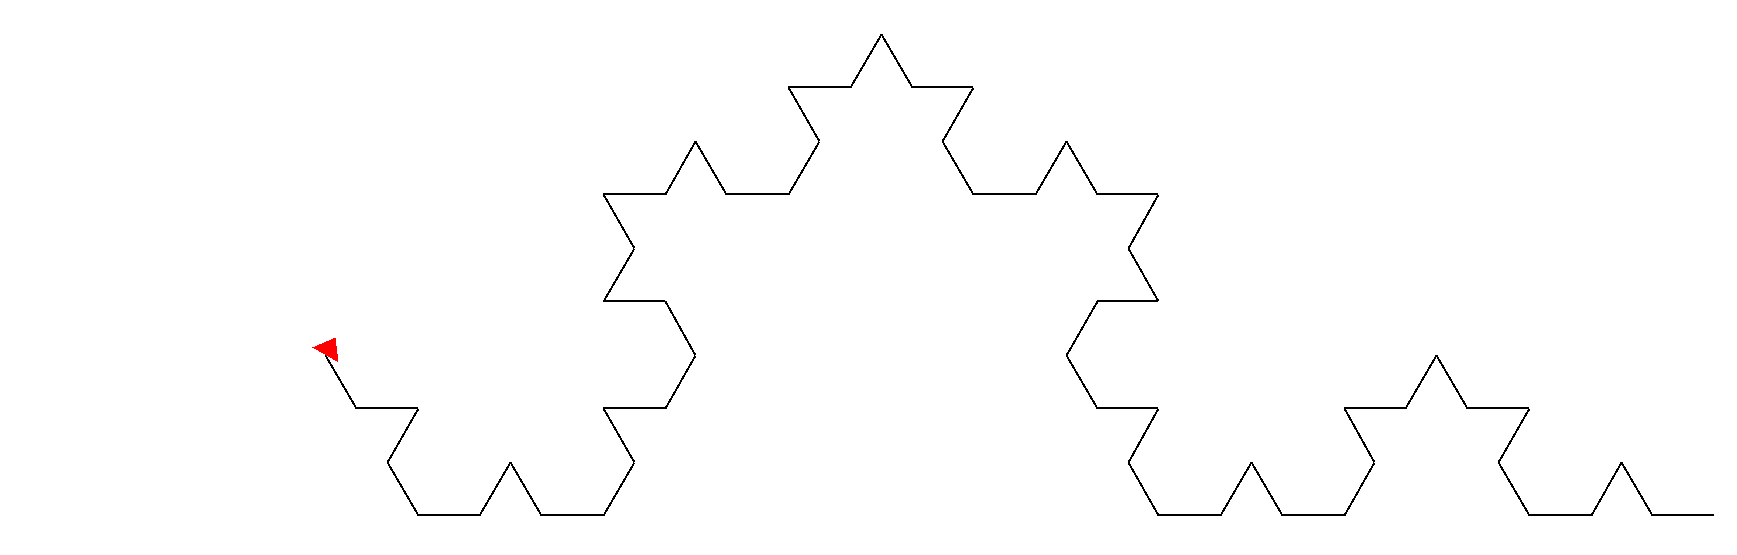
\includegraphics[width = \linewidth]{Thue-Morse Sequence/111.png}
		\caption{$n=111$}
	\end{subfigure}
	\begin{subfigure}{0.3\linewidth}
		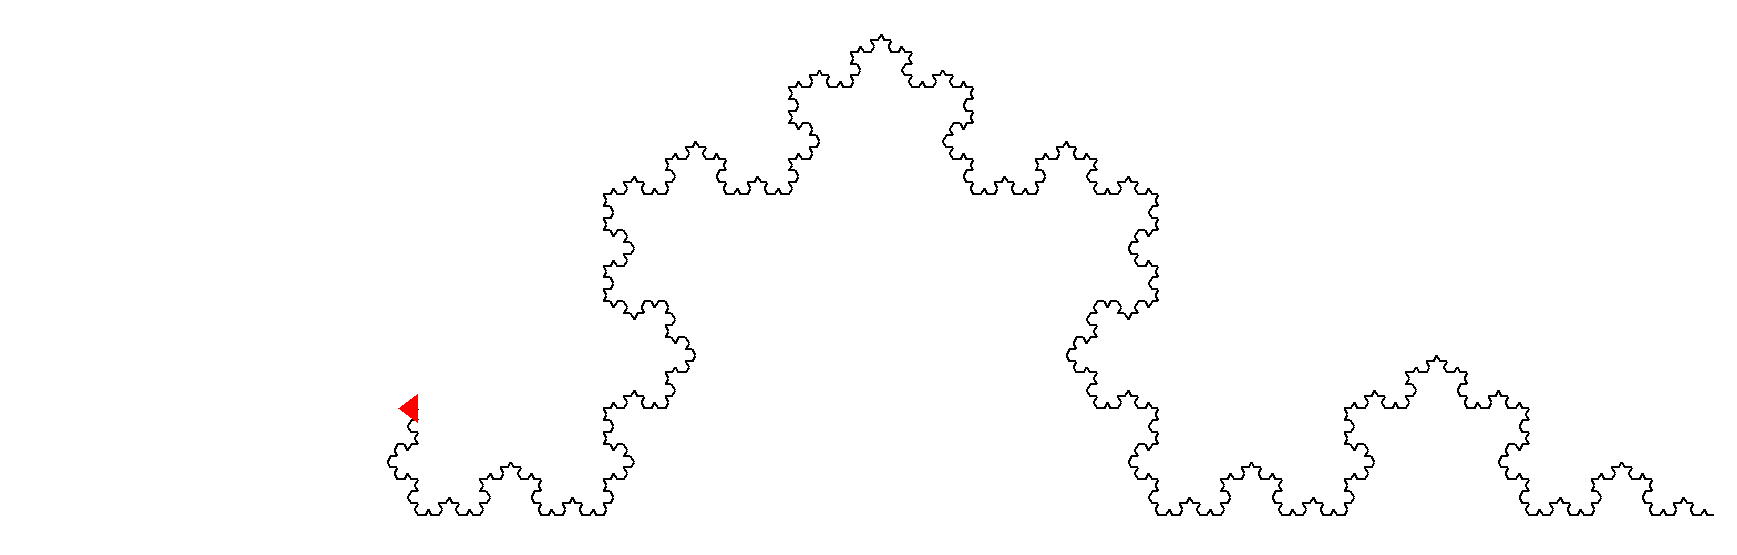
\includegraphics[width = \linewidth]{Thue-Morse Sequence/1729.png}
		\caption{$n=1729$}
	\end{subfigure}
	\caption{The outputs for numbers which are not a odd power of 2}
\end{figure}
\begin{funvideo}
	\href{https://youtu.be/prh72BLNjIk}{The Fairest Sharing Sequence Ever -- Stand-up Maths}\\
	\href{https://youtu.be/RU0wScIj36o}{Fractal charm: Space filling curves -- 3Blue1Brown}
\end{funvideo}
\KOMAoptions{paper=A4}
\recalctypearea